% !TeX root = ../main.tex
    \begin{frame}{Parameters Description}
      $M =4$, $\delta =1$, $|\Omega| = 1000$, $N =10$, $L_j =21, j \in \mathcal{N}$.
      
      \vspace{0.2cm}
      
      Consider three sets of probability distributions with the same expectation of demand each period:

      \vspace{0.2cm}

      \qquad D1: [0.25, 0.25, 0.25, 0.25]

      \vspace{0.2cm}

      \qquad D2: [0.25, 0.35, 0.05, 0.35]
      \vspace{0.2cm}

      \qquad D3: [0.15, 0.25, 0.55, 0.05]

      \vspace{0.2cm}

      Each entry in the result columns is the average of 100 instances.
    \end{frame}

    \begin{frame}{Performances of Different Policies}
        \scriptsize
        \begin{table}[ht]
          \centering
          \begin{tabular}{|c|c|c|c|c|c|c|}
          \hline
          Distribution & T & DSA (\%) & DP1 (\%) & Bid (\%) & Booking (\%) & FCFS (\%) \\
          \hline
          \multirow{5}{*}{D1} & 60   & {\color{red}99.12} & 98.42 & 98.38 & 96.74 & 98.17 \\
          & 70    & {\color{red}98.34} & 96.87 & 96.24 & 97.18 & 94.75 \\
          & 80    & {\color{red}98.61} & 95.69 & 96.02 & 98.00 & 93.18 \\
          & 90    & {\color{red}99.10} & 96.05 & 96.41 & 98.31 & 92.48 \\
          & 100   & {\color{red}99.58} & 95.09 & 96.88 & 98.70 & 92.54 \\
          \hline
          \multirow{5}{*}{D2} & 60   &  {\color{red}98.94} & 98.26 & 98.25 & 96.74 & 98.62 \\
             & 70   & {\color{red}98.05} & 96.62 & 96.06 & 96.90 & 93.96 \\
             & 80   & {\color{red}98.37} & 96.01 & 95.89 & 97.75 & 92.88 \\
             & 90   & {\color{red}99.01} & 96.77 & 96.62 & 98.42 & 92.46 \\
             & 100  & {\color{red}99.23} & 97.04 & 97.14 & 98.67 & 92.00 \\
          \hline
          \multirow{5}{*}{D3} & 60  &  {\color{red}99.14} & 98.72 & 98.74 & 96.61 & 98.07 \\
             & 70  & {\color{red}99.30} & 96.38 & 96.90 & 97.88 & 96.25 \\
             & 80  & {\color{red}99.59} & 97.75 & 97.87 & 98.55 & 95.81 \\
             & 90  & {\color{red}99.53} & 98.45 & 98.69 & 98.81 & 95.50 \\
             & 100 & {\color{red}99.47} & 98.62 & 98.94 & 98.90 & 95.25 \\
          \hline
          \end{tabular}
        \end{table}
        DSA has better performance than other policies under different demands.

    \end{frame}
      
    \begin{frame}{Impact of Social Distancing As Demand Increases}
      \vspace{-0.4cm}
      % \begin{figure}[h]
      %   \centering
      %   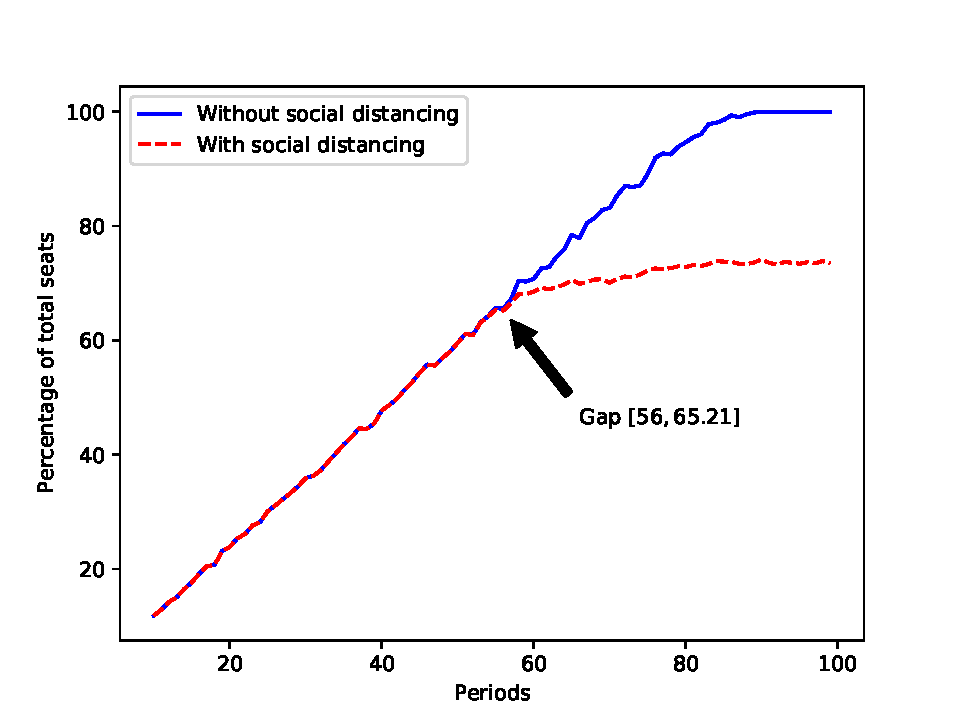
\includegraphics[width=0.5\textwidth]{./images/p1.pdf}          
      %   \caption{When probability is [0.25, 0.25, 0.25, 0.25]}
      %   \end{figure}
      \scriptsize
      When the probability distribution is $[0.25, 0.25, 0.25, 0.25]$
      \begin{columns}
        \column{6cm}  %第一栏(左栏)宽度为5cm
          \begin{figure}[ht]
            \centering
            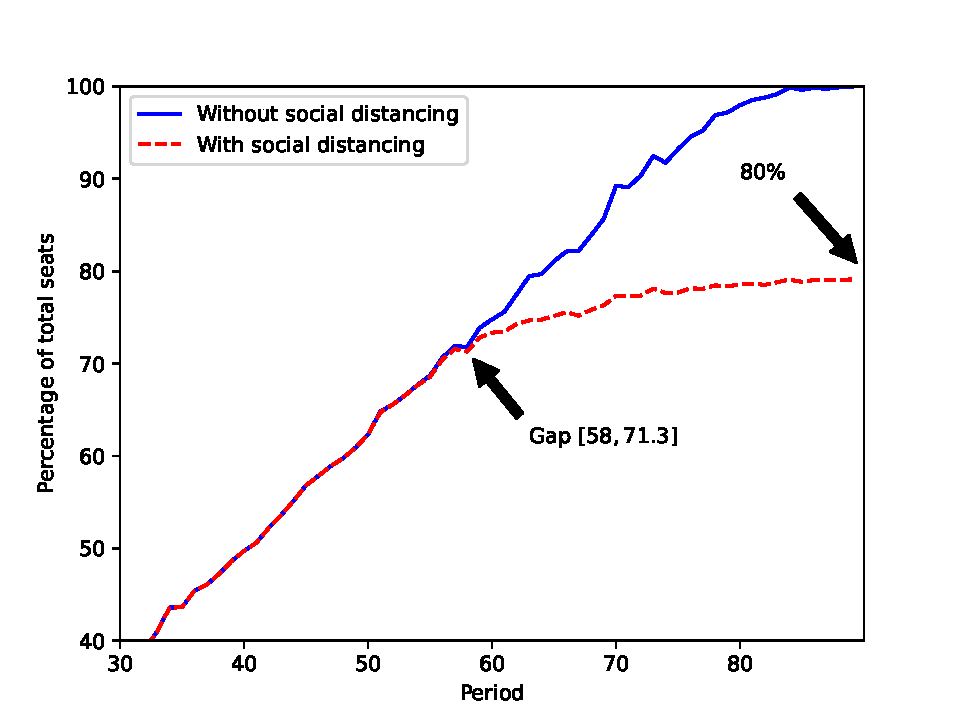
\includegraphics[width = 1\textwidth]{./images/without3.pdf}
          \end{figure}
          \column{6cm}
          \scriptsize
          \begin{figure}[ht]
            \centering
            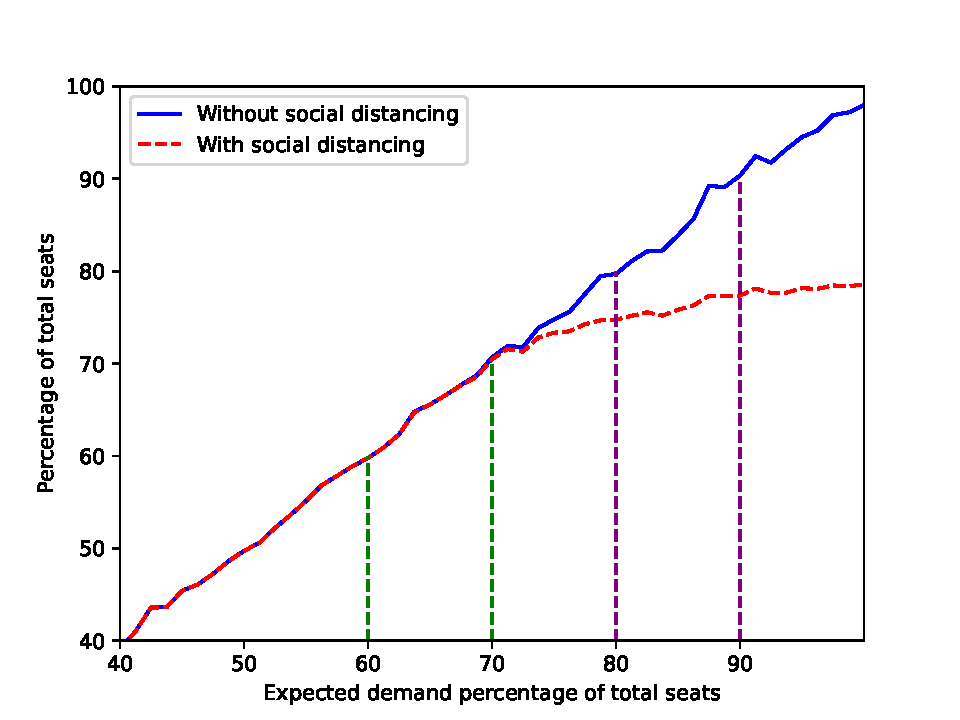
\includegraphics[width = 1\textwidth]{./images/without5.pdf}
          \end{figure}
      \end{columns}
      % The gap point represents the first period where the number of people without social distancing is larger than that with social distancing and the gap percentage is the corresponding percentage of total seats.
      \begin{itemize}
        \item Gap point: the first period when there is difference 
        \item Demand {\color{green}less than} 71.3\% total seats: no difference
        \item Demand {\color{violet}larger than} 71.3\% total seats: difference becomes larger
        \item The largest occupancy rate is 80\% by the property of the largest pattern.
      \end{itemize}
  \end{frame}

    \begin{frame}{Gap Points and Occupancy Rates under Different Probability Distributions}
      \scriptsize
      $\gamma = p_1 * 1 + p_2 * 2 + p_3 * 3 + p_4 * 4$: the expected number of people at each period.

      \begin{columns}
      \begin{column}{0.7\textwidth}
      
      \begin{figure}[ht]
        \centering
        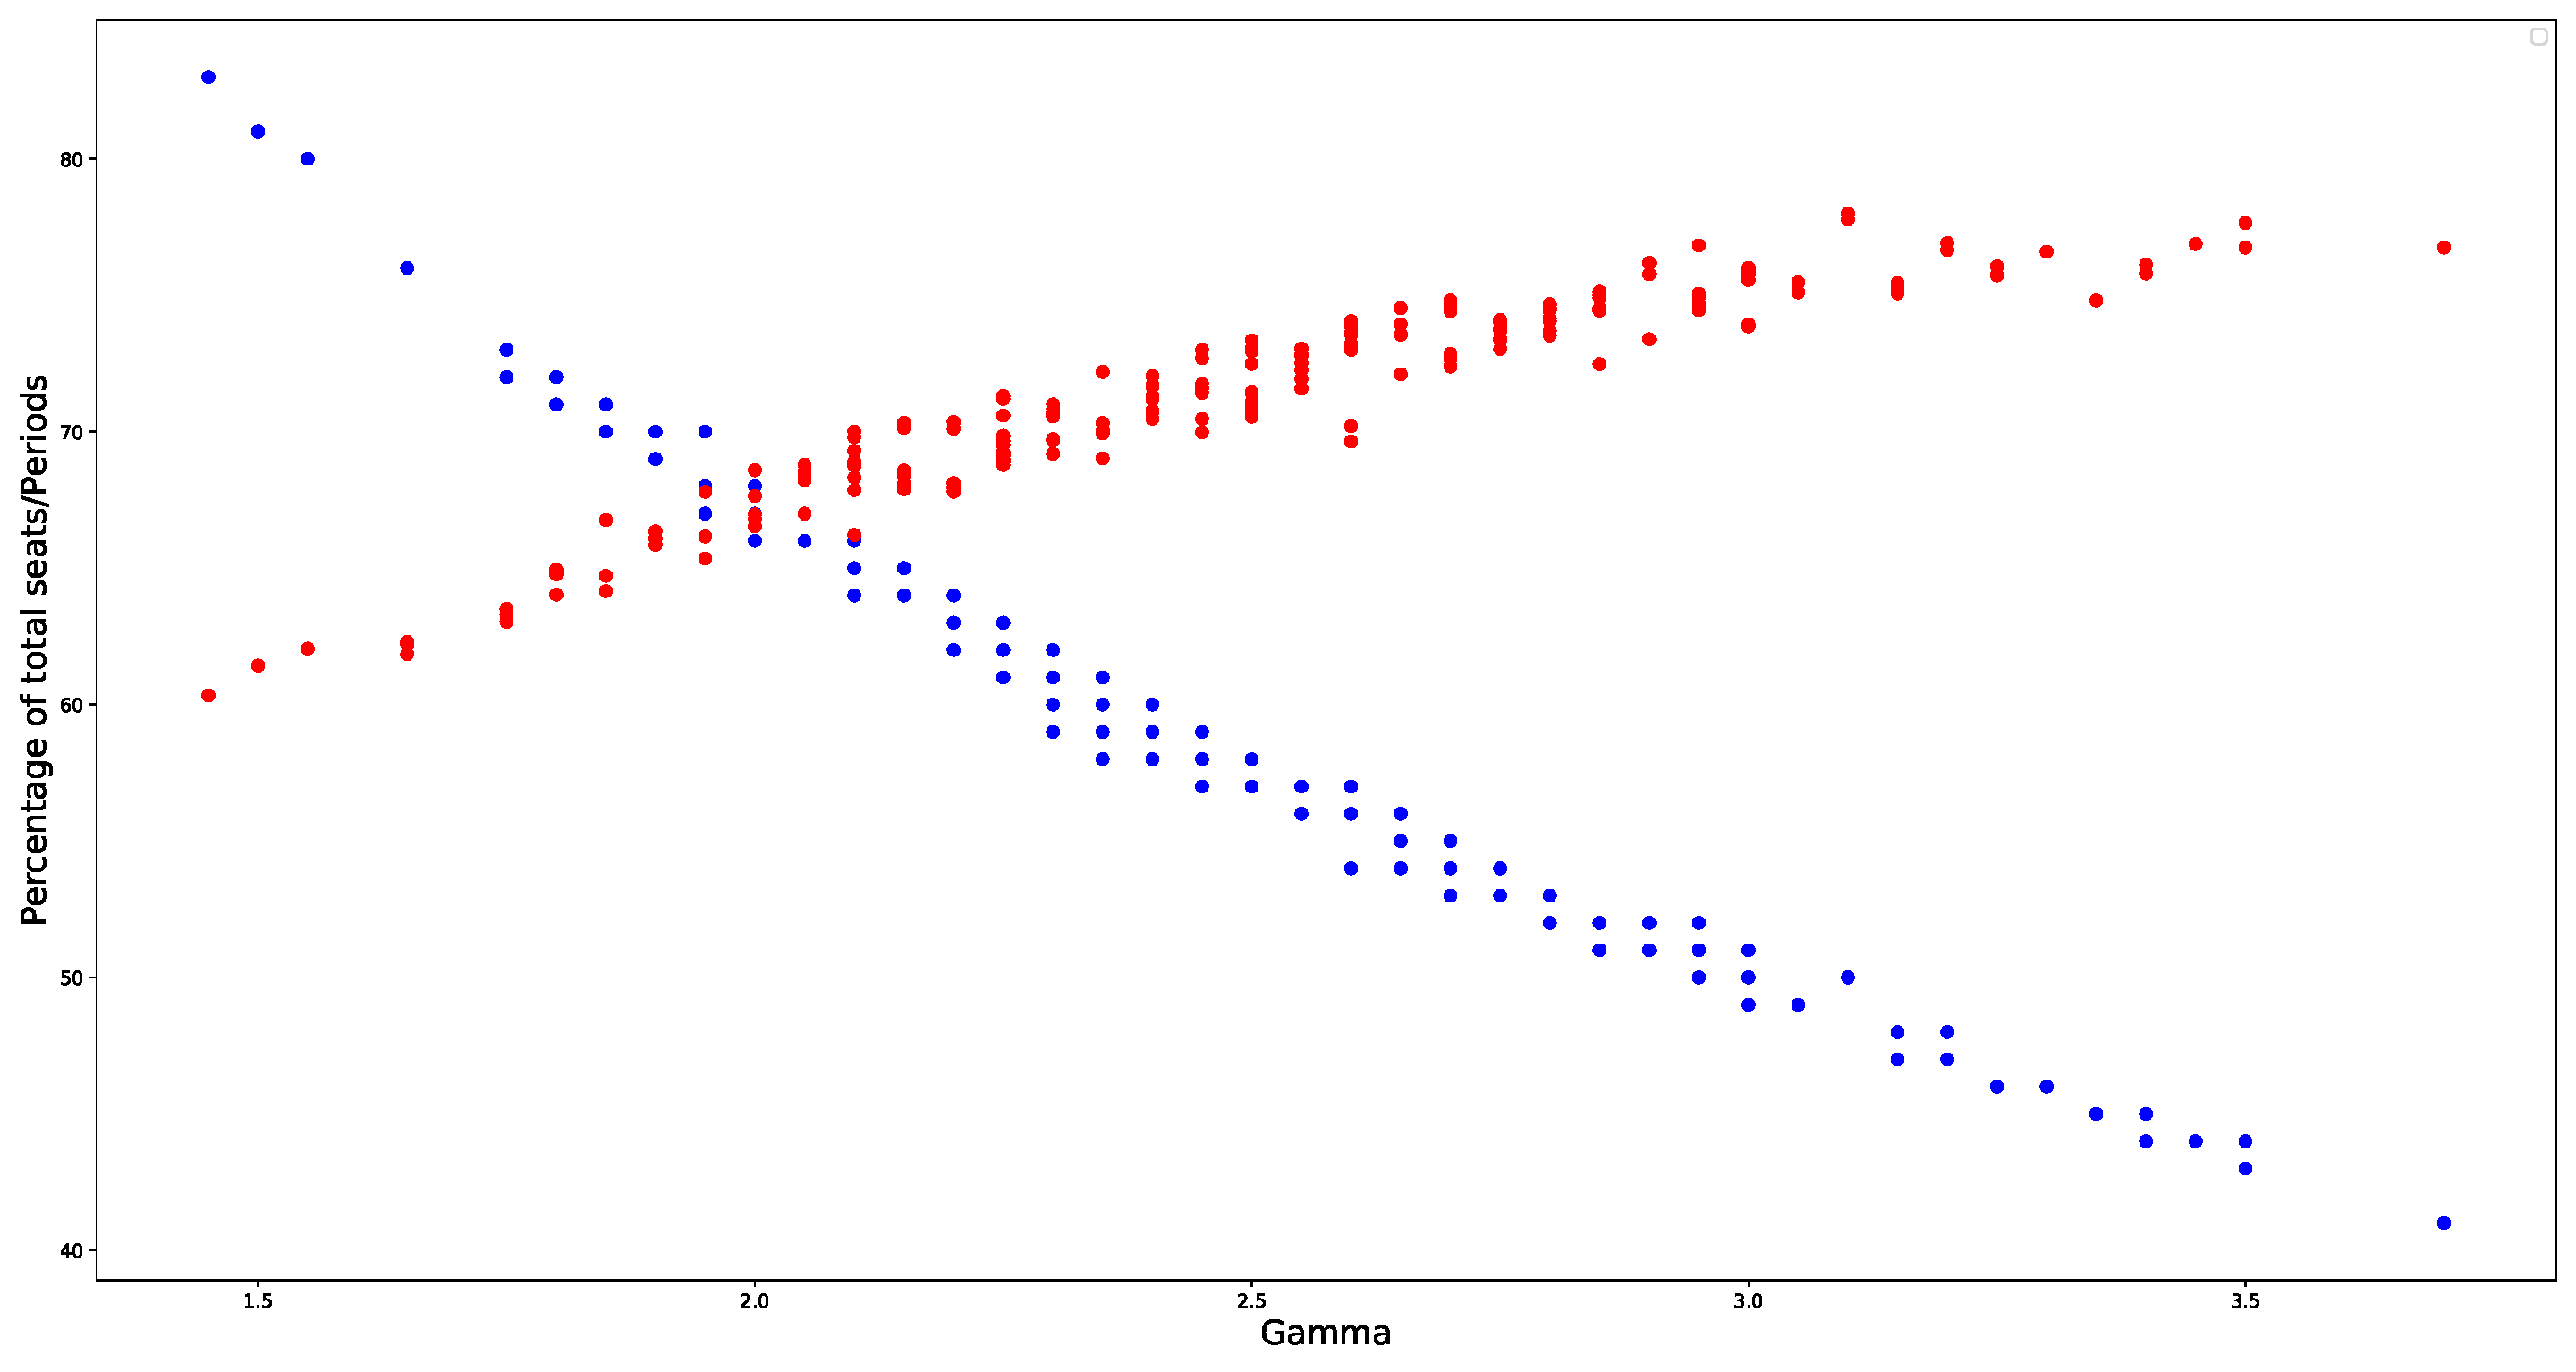
\includegraphics[width = 1\textwidth]{./images/gamma1.pdf}
        \captionsetup{font={scriptsize}}
        \caption{Gap points and occupancy rates with 200 probability distributions}
    \end{figure}
  \end{column}
    \begin{column}{0.3\textwidth}
    \scriptsize
    {\color{blue} Blue points}: period of the gap point.
      \vspace{0.2cm}

    {\color{red} Red points}: occupancy rate of the gap point. 
    \vspace{0.2cm}

    Difference is small under the same gamma.
  \end{column}
  \end{columns}
    \end{frame}

    \begin{frame}{Estimation of Gap Points}
      \scriptsize
      \vspace{-0.2cm}

      \begin{columns}
        \begin{column}{0.6\textwidth}
      \begin{figure}[ht]
        \centering
        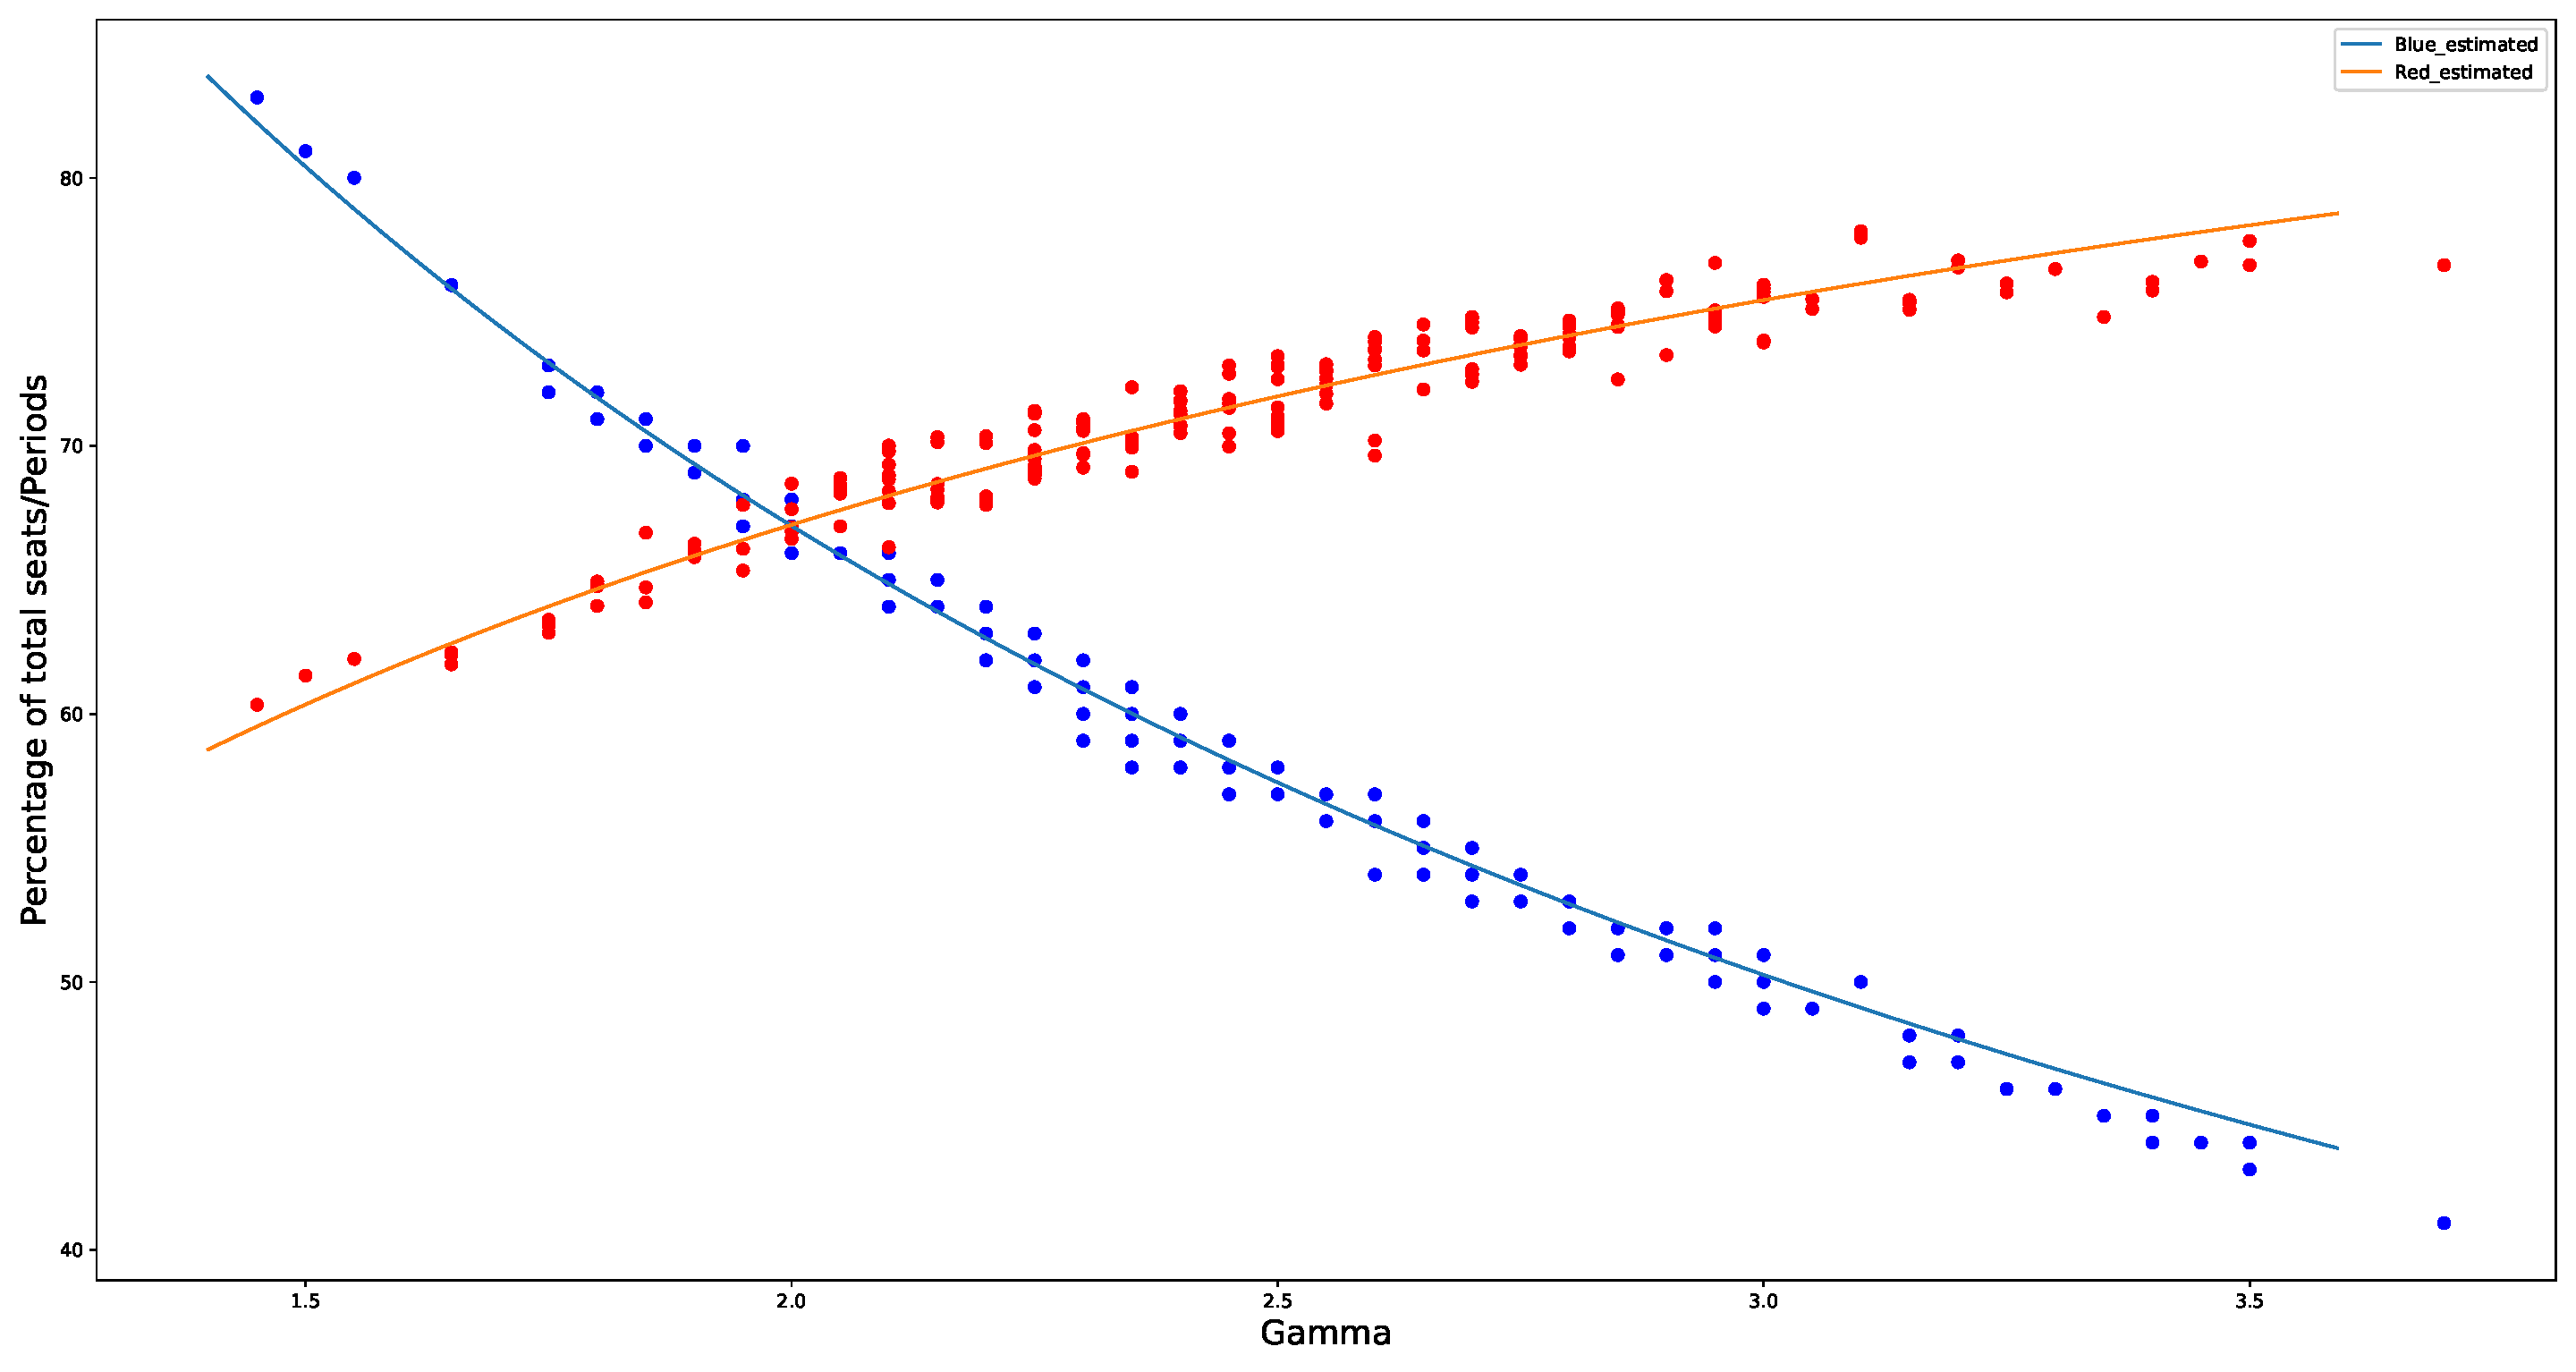
\includegraphics[width = 1\textwidth]{./images/gamma.pdf}
        % \captionsetup{font={scriptsize}}
        % \caption{Gap points and occupancy rates with 200 probability distributions}
    \end{figure}
  \end{column}

  \begin{column}{0.4\textwidth}
    Ideal: the groups before gap point will occupy all seats.
    $c_1, c_2$ can be seen as the discount factor compared to the ideal situation.

    Gap points can be estimated with $\gamma$.

    {\color{blue} $y_1 = \frac{c_1 \tilde{L}}{\gamma + \delta}$}, 
    {\color{red}  $y_2 = c_2 \frac{\gamma}{\gamma + \delta} \frac{\tilde{L}}{\tilde{L}-N \delta}$}

    The larger $c_1, c_2$, the closer to the ideal situation.
  \end{column}
  \end{columns}

    \scriptsize
    \begin{table}[ht]
      \centering
      % \caption{Fitting values of $c_1$ and $c_2$}
      \begin{tabular}{|c|c|c|}
      \hline
       Seat layout(\# of rows $\times$ \# of seats) & Fitting Values of $c_1$ & Fitting Values of $c_2$  \\
      \hline
       10 $\times$ 11 & 0.909 $\pm$ 0.013  & 89.89 $\pm$ 1.436 \\
       10 $\times$ 16 & 0.948 $\pm$ 0.008  & 94.69 $\pm$ 0.802 \\
       10 $\times$ 21 & 0.955 $\pm$ 0.004 & 95.44 $\pm$ 0.571 \\
       10 $\times$ 26 & 0.966 $\pm$ 0.004 & 96.23 $\pm$ 0.386 \\
       10 $\times$ 31 & 0.965 $\pm$ 0.003 & 96.67 $\pm$ 0.434 \\
       10 $\times$ 36 & 0.968 $\pm$ 0.003 & 97.04 $\pm$ 0.289 \\
       \hline
      \end{tabular}
    \end{table}
    
    The larger the size of row is, the larger the values of $c_1, c_2$ are. 
    
  
  \end{frame}
  %   \begin{frame}{Impact of Social Distancing as Demand Increases}


  % \end{frame}

    % We simulate 200 probabilities. For each probability, we run 100 instances to calculate the gap point and the corresponding occupancy rate on average. 
    
    % The point in the figure is the average of 100 instances.
    % x-axis is gamma, y-axis is periods/ and occupancy rate.

    % \begin{frame}{Seat Assignment under Fixed Seat Planning}
    %   % To evaluate the effectiveness of the initial seat planning, we employ a dynamic situation where decisions are made based on real-time feedback. In this context, we utilize a fixed seat planning as the foundation, and then make informed decisions accordingly.
    %   \small
    %   \begin{itemize}
    %     \item Group-type Control
    %     \item[-] Suppose the corresponding supply is $[X_1, \ldots, X_M]$. ($X_{i} = \sum_{j} x_{ij}, \forall i$)
        
    %     For the arrival of group type $i$,
  
    %     \item[-] if $X_i > 0$, accept it directly, assign it the seats planned for group type $i$;
    %     \item[-] if $X_i = 0$, determine which group type to accept it.
    %   \end{itemize}
  
    %   \vspace{-0.5cm}
  
    %   \begin{figure}[h]
    %     \centering
    %     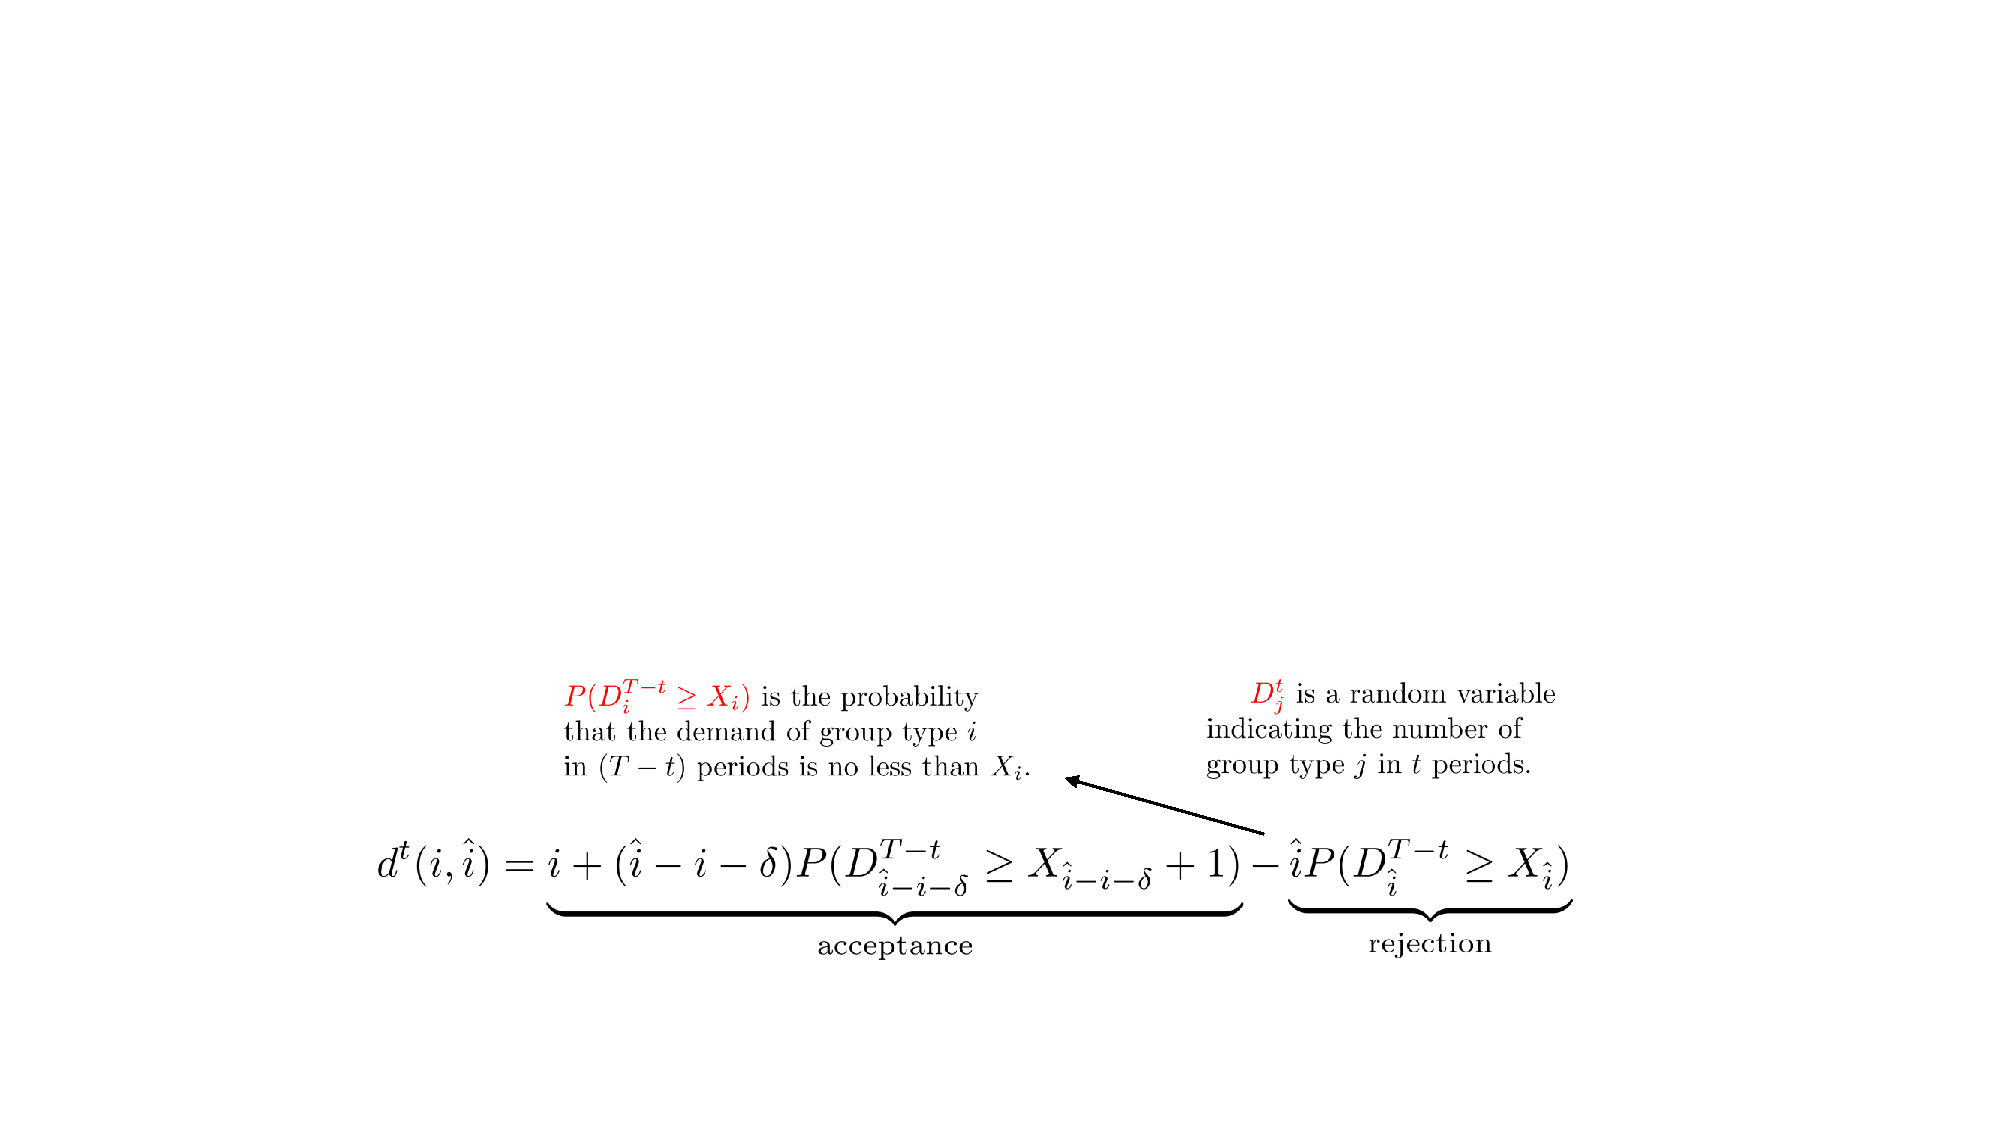
\includegraphics[width = 0.8\textwidth]{./images/group_type.pdf}
    %   \end{figure}
  
    %   \vspace{-0.1cm}
  
    %   For all $\hat{i} > i$, find the maximum value denoted as $d^{t}(i, \hat{i}^{*})$.
      
    %   If $d^{t}(i, \hat{i}^{*}) \geq 0$, we place the group of $i$ in $(\hat{i}^{*} + \delta)$-size seats. Otherwise, reject the group.
  
    %   % After acceptance, customers have more freedom to choose their seats with the seat planning.
    % \end{frame}

    % \begin{frame}{Seat Assignment After All Groups Arrive}
    %   This setting is particularly applicable to larger venues, such as stadiums, where an immediate decision is made when a group arrives, but the actual seat assignment for that group is deferred after all groups arrive.

    %   \vspace{0.5cm}

    %   The critical part is to make the decision, thus, we choose the following policies associated with relaxation forms.

    %   \vspace{0.5cm}

    %   Policies: 

    %   \begin{itemize}
    %     \item Dynamic programming based heuristic
    %     \item Bid-price control
    %   \end{itemize}
    % \end{frame}

      \begin{frame}{Seat Assignment After All Groups Arrive}
        \scriptsize
        DP1-A: Dynamic programming based heuristic policy after all groups arrive
        
        Bid-A: Bid-price control policy after all groups arrive
        \begin{table}[ht]
          \centering
          \begin{tabular}{|c|c|c|c|c|c|}
          \hline
          Distribution & T  & {\color{red}DP1-A} (\%) & {\color{red}Bid-A} (\%) & DP1 (\%) & Bid (\%) \\
          \hline
          \multirow{5}{*}{D1} & 60    & 99.52 & 99.44 & 98.42 & 98.38 \\
          & 70  &    99.32 & 98.97 & 96.87 & 96.24 \\
          & 80  &    99.34 & 99.30 & 95.69 & 96.02 \\
          & 90  &    99.55 & 99.49 & 96.05 & 96.41  \\
          & 100 &    99.78 & 99.66 & 95.09 & 96.88 \\
          \hline
          \multirow{5}{*}{D2} & 60   & 99.50 & 99.37 & 98.26 & 98.25  \\
          & 70  &   99.40 & 98.97 & 96.62 & 96.06 \\
          & 80  &    99.46 & 99.24 & 96.01 & 95.89 \\
          & 90  &    99.59 & 99.35 & 96.77 & 96.62 \\
          & 100 &    99.77 & 99.61 & 97.04 & 97.14  \\
          \hline
          \multirow{5}{*}{D3} & 60   & 99.57 & 99.54 & 98.72 & 98.74 \\
          & 70  &    99.46 & 99.39  & 96.38 & 96.90 \\
          & 80  &    99.50 & 99.30  & 97.75 & 97.87 \\
          & 90  &    99.34 & 99.44  & 98.45 & 98.69 \\
          & 100 &    99.34 & 99.55  & 98.62 & 98.94 \\
          \hline
          \end{tabular}
        \end{table}
      The performance is greatly improved without the assign-to-seat constraint.  
    \end{frame}

    \begin{frame}{Seat Assignment under Fixed Seat Planning}
      \scriptsize
      The assignment is based on the fixed seat planning and the group-type control.
      \begin{table}[ht]
        \centering
        \begin{tabular}{|c|c|c|c|}
        \hline
        Distribution & T &  \# of rows & Compared to the optimal (\%)  \\
        \hline
        \multirow{4}{*}{D1} & 70    & \multirow{4}{*}{10} & 94.97  \\
        & 80     &  & 96.48   \\
        & 90     &  & 97.94   \\
        & 100     &  & 98.91   \\
        \hline
        \multirow{4}{*}{D2} & 70    & \multirow{4}{*}{10} & 95.90 \\
        & 80     &  & 97.06  \\
        & 90     &  & 98.58  \\
        & 100     &  & 99.47 \\
        \hline
        \multirow{4}{*}{D3} & 70    & \multirow{4}{*}{10} & 97.41  \\
        & 80     &  & 98.85  \\
        & 90     &  & 98.73  \\
        & 100     &  & 98.46  \\
        \hline
        \multirow{4}{*}{D1} & 140   & \multirow{4}{*}{20} & 95.83  \\
        & 160     &  & 97.46  \\
        & 180     &  & 99.05  \\
        & 200    &  & 99.74  \\
        \hline
        \end{tabular}
      \end{table}
      The performance declines with the fixed seat planning constraint.
    \end{frame}